\subsection{态射}

在本节及下一节中，为简单起见，我们假定所考虑的结构物种只有一个基集（因此它是一个主基集）。读者不难将定义和结果推广到一般情形。

让 \(\Sigma\) 是理论中的一类结构 \(\mathcal{C}\) 它比集合论更强，并且设 \(x, y, s, t\) 是四个不同的字母，它们与以下常量不同 \(\mathcal{C}\) 。我们回顾一下记号 \(\mathcal{F}(x, y)\) 表示从 \(x\) 进入。 \(y\) (第二章，§5，第2节)。假设我们给定一个项 \(\sigma\{x, y, s, t\}\) 在 \(\mathcal{C}\) 满足以下条件：

(MO \(_{I}\) ) 关系“ \(s\) 是物种 \(\Sigma\) 在 \(x\) 上的一个结构，以及 \(t\) 是物种 \(\Sigma\) 在 \(y\) 上的一个结构”蕴含，在 \(\mathfrak{C}\)，关系 \(\sigma\{x,y,s,t\} \subset \mathcal{F}(x,y)\) .

\((\mathrm{MO}_{\mathrm{II}})\) 如果在某个理论中 \(\mathfrak{C}'\) 强于 \(\mathfrak{C}\) ，我们有三组集合 \(\mathbf{E}\) , \(\mathbf{E}'\) , \(\mathbf{E}''\) 分别配备了结构 \(\mathscr{S}\) , \(\mathscr{S}'\) , \(\mathscr{S}''\) 的物种 \(\Sigma\) ，则关系 \(f \in \sigma \{ \mathbf{E}, \mathbf{E}', \mathscr{S}, \mathscr{S}' \}\) 并且 \(g \in \sigma \{ \mathbf{E}', \mathbf{E}'', \mathscr{S}', \mathscr{S}'' \}\) 蕴含关系

\[
g \circ f \in \sigma \left\{\mathrm{E}, \mathrm{E} ^ {\prime \prime}, \mathscr {S}, \mathscr {S} ^ {\prime \prime} \right\}.
\]

\((\mathrm{MO}_{\mathrm{III}})\) 如果在某个理论中 \(\mathfrak{C}'\) 强于 \(\mathfrak{C}\) ，我们有两个集合 \(\mathbf{E}\) , \(\mathbf{E}'\) 分别配备了结构 \(\mathcal{S}\) , \(\mathcal{S}'\) 的物种 \(\Sigma\) ，则一个双射 \(f\) 的 \(\mathbf{E}\) 到上 \(\mathbf{E}'\) 是一个同构，当且仅当 \(f \in \sigma \left\{\mathbf{E}, \mathbf{E}', \mathcal{S}, \mathcal{S}'\right\}\) 并且 \(f^{-1} \in \sigma \left\{\mathbf{E}', \mathbf{E}, \mathcal{S}', \mathcal{S}\right\}\) .

如果 \(\Sigma\) 并且 \(\sigma\) 给定后，关系 \(f \in \sigma\{x, y, s, t\}\) 用以下说法来表达： \(f\) 是一个态射（或一个 \(\sigma\) -态射）从 \(x\) ，赋予 \(s\) 到 \(y\) ，赋予 \(t\) 。如果在某个理论中 \(\mathfrak{G}'\) 强于 \(\mathfrak{G}\) ) \(\mathbf{E}\) 并且 \(\mathbf{E}'\) 是两个配备了结构的集合 \(\mathcal{S}, \mathcal{S}'\) 的物种 \(\Sigma\) ，则项 \(\sigma\{\mathbf{E}, \mathbf{E}', \mathcal{S}, \mathcal{S}'\}\) 是 \(\sigma\) -态射的集合 \(\mathbf{E}\) 进入。 \(\mathbf{E}'\) .

示例

\begin{enumerate}
\def\labelenumi{(\arabic{enumi})}
\item
  取 \(\Sigma\) 为序结构的种类，并令 \(\sigma\{x, y, s, t\}\) 表示所有映射 \(f\) 所成的集合，其中每个映射都从 \(x\) 到 \(y\) ，并使关系 \((u, v) \in s\) 蕴含 \((f(u), f(v)) \in t\) 。按第三章第1节的记号，这意味着 \(u \leqslant v\) 蕴含 \(f(u) \leqslant f(v)\) ，即 \(f\) 是递增的。容易验证公理 \((\mathrm{MO}_{\mathbf{I}}), (\mathrm{MO}_{\mathbf{II}})\) 以及 \((\mathrm{MO}_{\mathbf{III}})\) 。
\item
  取 \(\Sigma\) 为一种代数结构，其只有一个处处有定义的（内部）合成律（§1，第4号，例2）。设 A, A' 是两个赋予种类 \(\Sigma\) 结构的集合， \(p, p'\) 是这两个结构的合成律。考虑从 A 到 A' 的映射 \(f\) ，它们满足 \(p'(f(x), f(y)) = f(p(x, y))\) ，对任意 \(x \in A\) 和任意 \(y \in A\) 都成立。这些映射满足 (MO \(_{I}\) ), (MO \(_{II}\) ）以及（MO \(_{III}\) ），称为从 A 到 A' 的同态。
\item
  取 \(\Sigma\) 为拓扑结构的种类（§1，第4号，例3）。设 A、A' 分别是赋予拓扑 V、V' 的两个集合。考虑从 A 到 A' 的映射 \(f\) ，使下述
\end{enumerate}

关系成立： \(\mathbf{X}' \in \mathbf{V}'\) 蕴含 \(\overline{f}^{1}(\mathbf{X}') \in \mathbf{V}\) （换言之，拓扑 \(\mathbf{V}'\) 中每个开集的原像都是拓扑 \(\mathbf{V}\) 中的开集）。这些映射满足 \((\mathrm{MO}_{\mathbf{I}})\) , \((\mathrm{MO}_{\mathbf{II}})\) 以及 \((\mathrm{MO}_{\mathbf{III}})\) ，它们就是从 \(\mathbf{A}\) 到 \(\mathbf{A}'\) 的连续映射（相对于拓扑 \(\mathbf{V}\) 和 \(\mathbf{V}'\) ）（参见《一般拓扑学》第一章第2节）。

注记。对于给定的结构种类 \(\Sigma\) ，有时需要定义不同的项 \(\sigma \{x, y, s, t\}\) ，但它们都满足条件 \((\mathrm{MO}_{\mathbf{I}})\) , \((\mathrm{MO}_{\mathbf{II}})\) 以及 \((\mathrm{MO}_{\mathbf{III}})\) 。例如，设 \(\Sigma\) 是拓扑结构的种类，并采用上面例3的记号。如果映射 \(f\) 从 A 到 \(\mathbf{A}'\) ，并使关系 \(\mathbf{X} \in \mathbf{V}\) 蕴含 \(f(\mathbf{X}) \in \mathbf{V}'\) （换言之， \(f\) 把每个开集的像都映为开集），则称它为开映射。容易验证，开映射也满足条件 \((\mathrm{MO}_{\mathbf{I}})\) , \((\mathrm{MO}_{\mathbf{II}})\) 以及 \((\mathrm{MO}_{\mathbf{III}})\) ，它们都是种类 \(\Sigma\) 的态射。* 此外，连续映射不一定是开映射，开映射也不一定连续。* 因此，一个给定的结构种类并不自然确定唯一的态射概念。

\pandocbounded{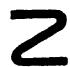
\includegraphics[keepaspectratio]{images/part002_a17f5ac5846160dabe35edfd7ae1b1f71cd54f2b9ab149a24f189ab7736ff1b5.jpg}}

凡涉及序结构、代数结构和拓扑结构时，除非另有明确说明，始终应理解为态射即为上述各例中所定义的态射。

条件 \((MO_{III})\) 且双射的刻画（第二章，§3，第8号，命题8的推论）蕴含以下准则：

CST8. 设 E、E' 为两个集合，每个集合都赋予一个 Σ 型结构。设 f 为从 E 到 E' 的 σ-态射，并设 g 为从 E' 到 E 的 σ-态射。若 g∘f 是 E 到其自身的恒等映射，且 f∘g 是 E' 到其自身的恒等映射，则 f 是 E 到 E' 的同构，且 g 是逆同构。

\pandocbounded{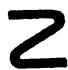
\includegraphics[keepaspectratio]{images/part002_4a2c9e6ca2e0232c08246aaeec85214d3ec9d06a429c17d5fe3c6f33ea15bbf4.jpg}}

应当指出，从E到E'的双射可能是一个σ-态射，而不必要求其逆双射也是σ-态射。* 例如，从拓扑空间A到拓扑空间A'的双射映射可以是连续的，而其逆双射不必是连续的（《一般拓扑学》，第一章，第2节，第1号，注记1）。*

备注。当一类结构 \(\Sigma\) 有多个主基集 \(x_{1},\ldots ,x_{n}\) ，以及辅助基集 \(\mathrm{A}_1,\dots ,\mathrm{A}_m\) ，一个 \(\sigma\) -态射是一个系统 \((f_1,\dots ,f_n)\) ，其中 \(f_{i}\) 是……的映射 \(x_{i}\) 进入。 \(y_{i}(1\leqslant i\leqslant n)\) ，并且这些映射系统满足与（MO \(_{\mathrm{II}}\) ) 和 (MO \(_{\mathrm{III}}\) )，读者可以很容易地自行陈述。

